\section{Rein. Learning}


TD learning makes nearby (in time) states have nearby values.

The TD $\lambda$ term controls how far back in time error feeds back from 0 to 1.

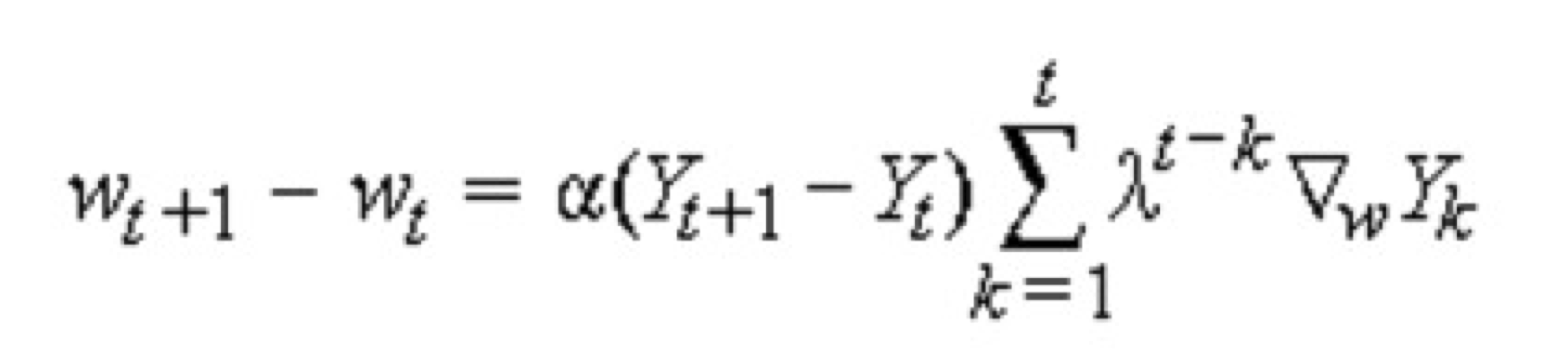
\includegraphics[width=0.9\columnwidth]{images/td}

Alpha go:

Had a policy and value network. Policy helps select paths in MCTS, value determines
$P(win)$ given current configuration.

Alpha go ZERO was not trained with any human data.

Policy: mapping from states to action $\pi_t(s,a) =$ probability that $a_t = a$ when $s_t = s$

\textbf{Exploration} ($\epsilon$) represents how explorative the RNN is.
